\documentclass[12pt,fleqn]{article}\usepackage{../common}
\begin{document}
Dinamik Programlama

Dinamik programlamanin (DP) temelinde ardi ardina verilmesi gereken
kararlarin bulunmasi fikri yatar; her anda, her verilen karar baska bir
karar secenekleri ortaya cikarabilir, ve bunlarin arasinda da secim
yapilmalidir. Hedefimiz en iyi karar zincirini bulmaktir. Bu kismen
``acgozlu algoritmalar (greedy algorithms)'' olarak bilinen algoritmalarin
yaptigina benzer, fakat acgozlu algoritmalar sadece ``o an icin' en iyisini
yapar; Fakat o an icin iyi olan toplam goze alindigi zaman en iyi sonucu
ortaya cikarmayabilir. Mesela alttaki grafige bir bakalim,

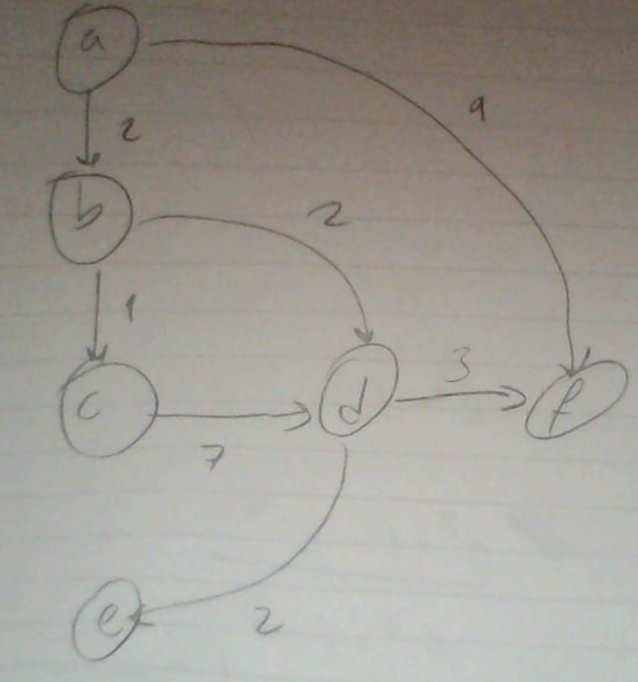
\includegraphics[height=6cm]{dp1.jpg}

Diyelim ki \verb!a! noktasindan \verb!f! noktasina en kisa yoldan ulasmaya
calisiyoruz. Acgozlu algoritma \verb!a,b,c,d! uzerinden gidis yapardi cunku
her an, sadece ``o an icin'' en iyi olani secerdi. Fakat toplama bakarsak,
bu yolun en kisa yol olmadigini goruruz. En iyi yol \verb!a,b,d! uzerinden
giden yoldur.

Ustteki cizit, ag yapisi (graph) yonlu, �evrimsiz (directed, acyclic graph
-DAG-) diye bilinen bir yapidir. Tipik kisa yol problemleri bu yapilar
uzerinde calisirlar. 

DP problemleri bir problemi alt problemlere bolebildigimiz zaman
faydalidirlar ve ozellikle o alt problemler cogunlukla tekrar tekrar
hesaplaniyorlarsa iyidir, cunku DP o alt problemleri onbellekleyerek tekrar
hesaplanmadan gecilmelerini saglayabilir. 

Ornek olarak en kisa yol problemini DP ile cozelim. 

Problemin tamami, teorik ve tumevarimsal olarak biraz dusunelim. Diyelim ki
ustteki DAG'de $a,f$ arasindaki en kisa yolu biliyoruz. Ve yine diyelim ki
bu yol uzerinde / bir ara nokta $x$ noktasi var. O zaman, $a,x$, ve $x,f$
arasindaki yollar da tanim itibariyle en kisadir. Ispat: eger mesela $x,f$
arasindaki en kisa yol bildigimizden baska olsaydi, o zaman eldekini atip o
yolu kullaniyor olurduk, ve bu sefer bu alternatif en kisa olurdu. Fakat
ilk basta en kisa yolu bildigimiz faraziyesi ile basladik. Bir celiski elde
ettik, demek ki ara noktanin kisaligi dogrudur $\square$


Oyle bir fonksiyon $d(v)$ olsun ki herhangi bir $v$ nodu icin o nod'dan
bitis noktasina olan uzakligi hesapliyor olsun, $u,v$ arasindaki mesafe ise
$w(u,v)$ ile verilecek.

\begin{minted}{python}
DAG = {
    'a': {'b':2, 'f': 9},
    'b': {'d':2, 'c':1, 'f': 6},
    'c': {'d':7},
    'd': {'e':2, 'f': 3},
    'e': {'f':4},
    'f': {}
}
\end{minted}

En kisa yolu bulacak program

\begin{minted}{python}
from functools import wraps

def memo(func):
    cache = {}                                  
    @wraps(func)                                
    def wrap(*args):                            
        if args not in cache:
            print 'miss', args[0]
            cache[args] = func(*args)
        else: print 'hit for', args[0]
        return cache[args]                      
    return wrap 

def rec_dag_sp(W, s, t): 
    @memo                                    
    def d(u):
        print ('At ' + u[0])
        if u == t: return 0                     
        dist = min(W[u][v]+d(v) for v in W[u])  
        print 'rewinding from',u,'dist=',dist
        return dist
    return d(s)                                 

dist = rec_dag_sp(DAG, 'a', 'f')
print 'uzaklik=', dist
\end{minted}

\begin{verbatim}
miss a
At a
miss b
At b
miss c
At c
miss d
At d
miss e
At e
miss f
At f
rewinding from e dist= 4
hit for f
rewinding from d dist= 3
rewinding from c dist= 10
hit for d
hit for f
rewinding from b dist= 5
hit for f
rewinding from a dist= 7
uzaklik= 7
\end{verbatim}

\end{document}
